\chapter{Estruturas de Lewis e geometria das moléculas}\label{ch:g10:lewis-and-shape}

Uma \omterm{def:g7:atoms-and-molecules:molecule}{molécula} de dióxido de carbono é linear; uma \omterm{def:g7:atoms-and-molecules:molecule}{molécula} de água é
angular. Essa única diferença de forma é uma das razões pelas quais a
água, com \omterm{def:g7:atoms-and-molecules:molecule}{moléculas} mais leves que as do dióxido de carbono, é líquida à
temperatura ambiente, enquanto o dióxido de carbono é um gás. Os \omterm{def:g7:atoms-and-molecules:atom}{átomos}
de uma \omterm{def:g7:atoms-and-molecules:molecule}{molécula} são mantidos juntos por \omterm{def:g9:inside-the-atom:nucleus}{elétrons} compartilhados, e o modo
como os \omterm{def:g9:inside-the-atom:nucleus}{elétrons} são compartilhados decide a forma. Este capítulo
desenha os \omterm{def:g9:inside-the-atom:nucleus}{elétrons} compartilhados e, a partir deles, prevê a forma.

\begin{recall}
Os \omterm{def:g10:electron-shells:valence}{elétrons de valência} são os da \omterm{def:g10:electron-shells:configuration}{camada} externa; os \omterm{def:g7:atoms-and-molecules:atom}{átomos} tendem a
alcançar a configuração de um \omterm{def:g10:electron-shells:family}{gás nobre}, oito \omterm{def:g9:inside-the-atom:nucleus}{elétrons} na \omterm{def:g10:electron-shells:configuration}{camada} externa
(\omterm{def:g10:electron-shells:octet}{regra do octeto}) ou dois para o hidrogênio (\omterm{def:g10:electron-shells:octet}{regra do dueto})
(\cref{ch:g10:electron-shells}). Os modelos moleculares representam os
\omterm{def:g7:atoms-and-molecules:atom}{átomos} por bolas e as ligações por varetas
(\cref{ch:g7:atoms-and-molecules}).
\end{recall}

\section{A ligação covalente}

\begin{definition}[Ligação covalente]\label{def:g10:lewis-and-shape:covalent-bond}
Uma \emph{ligação covalente}\index{ligacao covalente@ligação covalente} é um par de
\omterm{def:g9:inside-the-atom:nucleus}{elétrons} compartilhado por dois \omterm{def:g7:atoms-and-molecules:atom}{átomos}; em geral, cada \omterm{def:g7:atoms-and-molecules:atom}{átomo} fornece um
\omterm{def:g9:inside-the-atom:nucleus}{elétron} do par. Os dois \omterm{def:g7:atoms-and-molecules:atom}{átomos} contam o par compartilhado na sua \omterm{def:g10:electron-shells:configuration}{camada}
externa, o que permite aos dois alcançar um dueto ou um octeto.
\end{definition}

\begin{definition}[Pares ligantes e pares não ligantes]\label{def:g10:lewis-and-shape:lone-pair}
Numa \omterm{def:g7:atoms-and-molecules:molecule}{molécula}, os \omterm{def:g10:electron-shells:valence}{elétrons de valência} de cada \omterm{def:g7:atoms-and-molecules:atom}{átomo} estão agrupados em
pares. Um \emph{par ligante}\index{par ligante} é compartilhado entre
dois \omterm{def:g7:atoms-and-molecules:atom}{átomos} e forma uma \omterm{def:g10:lewis-and-shape:covalent-bond}{ligação covalente}; um \emph{par não
ligante}\index{par nao ligante@par não ligante} pertence a um só \omterm{def:g7:atoms-and-molecules:atom}{átomo} e não participa de
nenhuma ligação.
\end{definition}

\begin{proposition}[Quantas ligações um átomo forma]\label{prop:g10:lewis-and-shape:valence}
Um \omterm{def:g7:atoms-and-molecules:atom}{átomo} forma tantas \omterm{def:g10:lewis-and-shape:covalent-bond}{ligações covalentes} quantos \omterm{def:g9:inside-the-atom:nucleus}{elétrons} lhe faltam
para completar o seu dueto ou o seu octeto:
\begin{center}
\small
\begin{tabular}{lcccc}
\hline
\omterm{def:g7:atoms-and-molecules:atom}{átomo} & \omterm{def:g10:electron-shells:valence}{elétrons de valência} & ligações & \omterm{def:g10:lewis-and-shape:lone-pair}{pares não ligantes} & exemplo \\
\hline
H & 1 & 1 & 0 & \ce{H2} \\
C & 4 & 4 & 0 & \ce{CH4} \\
N & 5 & 3 & 1 & \ce{NH3} \\
O & 6 & 2 & 2 & \ce{H2O} \\
Cl & 7 & 1 & 3 & \ce{HCl} \\
\hline
\end{tabular}
\end{center}
\end{proposition}

\section{As estruturas de Lewis}

\begin{definition}[Estrutura de Lewis]\label{def:g10:lewis-and-shape:lewis-structure}
A \emph{estrutura de Lewis}\index{estrutura de Lewis} de uma \omterm{def:g7:atoms-and-molecules:molecule}{molécula}
representa os seus \omterm{def:g7:atoms-and-molecules:atom}{átomos} pelos símbolos, cada \omterm{def:g10:lewis-and-shape:lone-pair}{par ligante} por um traço
entre dois \omterm{def:g7:atoms-and-molecules:atom}{átomos} e cada \omterm{def:g10:lewis-and-shape:lone-pair}{par não ligante} por um par de pontos ao lado do
seu \omterm{def:g7:atoms-and-molecules:atom}{átomo}.
\end{definition}

\begin{definition}[Ligações duplas e triplas]\label{def:g10:lewis-and-shape:multiple-bond}
Dois \omterm{def:g7:atoms-and-molecules:atom}{átomos} podem compartilhar dois pares de \omterm{def:g9:inside-the-atom:nucleus}{elétrons}, uma
\emph{ligação dupla}\index{ligacao dupla@ligação dupla}, desenhada como dois traços, ou
três pares, uma \emph{ligação tripla}\index{ligacao tripla@ligação tripla}, desenhada
como três traços.
\end{definition}

\begin{method}[Desenhar uma estrutura de Lewis]\label{met:g10:lewis-and-shape:draw}
\begin{enumerate}
  \item Some os \omterm{def:g10:electron-shells:valence}{elétrons de valência} de todos os \omterm{def:g7:atoms-and-molecules:atom}{átomos} e divida por dois
        para obter o número de pares.
  \item Ligue os \omterm{def:g7:atoms-and-molecules:atom}{átomos} por ligações simples (o hidrogênio, que forma uma
        ligação, fica sempre na periferia; o carbono em geral fica no
        centro).
  \item Distribua os pares restantes como \omterm{def:g10:lewis-and-shape:lone-pair}{pares não ligantes}, primeiro
        nos \omterm{def:g7:atoms-and-molecules:atom}{átomos} periféricos, para completar os seus octetos.
  \item Se um \omterm{def:g7:atoms-and-molecules:atom}{átomo} ainda não tiver octeto, transforme um \omterm{def:g10:lewis-and-shape:lone-pair}{par não ligante}
        de um vizinho num segundo (ou terceiro) par compartilhado.
  \item Verifique: cada hidrogênio tem 2 \omterm{def:g9:inside-the-atom:nucleus}{elétrons}, cada um dos outros
        \omterm{def:g7:atoms-and-molecules:atom}{átomos} tem 8, e todos os pares foram usados.
\end{enumerate}
\end{method}

\begin{example}[O dióxido de carbono]\label{ex:g10:lewis-and-shape:co2}
\ce{CO2}: $4 + 2 \times 6 = 16$ \omterm{def:g10:electron-shells:valence}{elétrons de valência}, 8 pares. As
ligações simples \ce{O-C-O} usam 2 pares; 6 \omterm{def:g10:lewis-and-shape:lone-pair}{pares não ligantes} nos
oxigênios os completam, mas o carbono fica então com só 4 \omterm{def:g9:inside-the-atom:nucleus}{elétrons}.
Transformar um \omterm{def:g10:lewis-and-shape:lone-pair}{par não ligante} de cada oxigênio num par compartilhado dá
duas \omterm{def:g10:lewis-and-shape:multiple-bond}{ligações duplas}: agora cada \omterm{def:g7:atoms-and-molecules:atom}{átomo} tem um octeto.
\end{example}

\begin{omfigure}
\setchemfig{atom sep=2.0em}
\begin{tabular}{cccccc}
\chemfig{H-H} & \chemfig{H-\charge{0=\:,90=\:,270=\:}{Cl}} & \chemfig{H-\charge{90=\:,270=\:}{O}-H} &
\chemfig{H-\charge{90=\:}{N}(-[6]H)-H} & \chemfig{H-C(-[2]H)(-[6]H)-H} &
\chemfig{\charge{135=\:,225=\:}{O}=C=\charge{45=\:,315=\:}{O}} \\[4pt]
\small \ce{H2} & \small \ce{HCl} & \small \ce{H2O} & \small \ce{NH3} & \small \ce{CH4} & \small \ce{CO2} \\[10pt]
\chemfig{\charge{180=\:}{N}~\charge{0=\:}{N}} & \chemfig{\charge{135=\:,225=\:}{O}=\charge{45=\:,315=\:}{O}} &
\chemfig{C(-[3]H)(-[5]H)=C(-[1]H)-[7]H} & \chemfig{H-C~\charge{0=\:}{N}} &
\chemfig{H-C(-[6]H)=\charge{45=\:,315=\:}{O}} & \\[4pt]
\small \ce{N2} & \small \ce{O2} & \small \ce{C2H4} & \small \ce{HCN} & \small metanal \ce{CH2O} &
\end{tabular}

{\small \omterm{def:g10:lewis-and-shape:lewis-structure}{Estruturas de Lewis} de onze \omterm{def:g7:atoms-and-molecules:molecule}{moléculas}. Todo \omterm{def:g7:atoms-and-molecules:atom}{átomo} que não é
hidrogênio está cercado por quatro pares (ligações e \omterm{def:g10:lewis-and-shape:lone-pair}{pares não
ligantes}): um octeto.}
\end{omfigure}

\section{A geometria das moléculas}

\begin{proposition}[Os pares de elétrons ficam o mais afastados possível]\label{prop:g10:lewis-and-shape:shape}
Em volta de um \omterm{def:g7:atoms-and-molecules:atom}{átomo} central, os grupos de \omterm{def:g9:inside-the-atom:nucleus}{elétrons} --- cada ligação
simples, dupla ou tripla, e cada \omterm{def:g10:lewis-and-shape:lone-pair}{par não ligante} --- se repelem e se
dispõem o mais longe possível uns dos outros. A geometria da \omterm{def:g7:atoms-and-molecules:molecule}{molécula}
decorre disso:
\begin{center}
\small
\begin{tabular}{llll}
\hline
grupos em volta & dos quais \omterm{def:g10:lewis-and-shape:lone-pair}{pares não ligantes} & geometria & exemplo \\
\hline
2 & 0 & linear, ângulo \ang{180} & \ce{CO2}, \ce{HCN} \\
3 & 0 & trigonal plana, ângulo \ang{120} & \ce{CH2O}, \ce{C2H4} \\
4 & 0 & tetraédrica, ângulo \ang{109.5} & \ce{CH4} \\
4 & 1 & piramidal & \ce{NH3} \\
4 & 2 & angular & \ce{H2O} \\
\hline
\end{tabular}
\end{center}
\end{proposition}
\admitted

\begin{remark}[De onde vem isso]\label{rem:g10:lewis-and-shape:vsepr}
Essa regra é um modelo, e ela funciona notavelmente bem para as
\omterm{def:g7:atoms-and-molecules:molecule}{moléculas} pequenas; ela é tornada precisa, e em parte explicada, no
volume do primeiro ano da universidade. Os \omterm{def:g10:lewis-and-shape:lone-pair}{pares não ligantes} ocupam um
pouco mais de espaço que os \omterm{def:g10:lewis-and-shape:lone-pair}{pares ligantes}: o ângulo da amônia
(\ang{106.7}) e o da água (\ang{104.5}) são um pouco menores que os
\ang{109.5} do metano.
\end{remark}

\begin{omfigure}
\begin{tikzpicture}[font=\small]
  % methane, tetrahedral, in perspective
  \begin{scope}
    \node[aC] (c) at (0,0) {};
    \node[aH, minimum size=3.6mm] (hb) at (0.3,-0.12) {};
    \node[aH] (h1) at (0,1.05) {};
    \node[aH] (h2) at (-1.0,-0.45) {};
    \node[aH] (h3) at (0.72,-0.5) {};
    \begin{scope}[on background layer]
      \foreach \h in {h1,h2,h3,hb} \draw[bond] (c.center) -- (\h.center);
    \end{scope}
    \node[aC] at (0,0) {};
    \node at (0,-1.35) {metano: tetraédrica};
    \node[font=\footnotesize] at (-0.55,0.55) {\ang{109.5}};
  \end{scope}
  % ammonia, pyramid
  \begin{scope}[xshift=4.2cm]
    \fill[omDef!25] (0,0.2) ellipse (0.18 and 0.45);
    \node[font=\scriptsize, omDef] at (0,1.0) {par não ligante};
    \node[aN] (n) at (0,0) {};
    \node[aH] (h1) at (-0.95,-0.5) {};
    \node[aH] (h2) at (0.7,-0.55) {};
    \node[aH, minimum size=3.6mm] (h3) at (0.25,-0.2) {};
    \begin{scope}[on background layer]
      \foreach \h in {h1,h2,h3} \draw[bond] (n.center) -- (\h.center);
    \end{scope}
    \node[aN] at (0,0) {};
    \node at (0,-1.35) {amônia: piramidal};
  \end{scope}
  % water, bent
  \begin{scope}[xshift=8.4cm]
    \fill[omDef!25, rotate=25] (0,0.2) ellipse (0.16 and 0.42);
    \fill[omDef!25, rotate=-25] (0,0.2) ellipse (0.16 and 0.42);
    \node[aO] (o) at (0,0) {};
    \node[aH] (h1) at (-0.8,-0.58) {};
    \node[aH] (h2) at (0.8,-0.58) {};
    \begin{scope}[on background layer]
      \draw[bond] (o.center) -- (h1.center); \draw[bond] (o.center) -- (h2.center);
    \end{scope}
    \node[aO] at (0,0) {};
    \draw[black!60] (-0.32,-0.23) arc[start angle=216, end angle=324, radius=0.4];
    \node[font=\footnotesize] at (0,-0.65) {\ang{104.5}};
    \node at (0,-1.35) {água: angular};
  \end{scope}
  % carbon dioxide, linear
  \begin{scope}[xshift=12.0cm]
    \node[aO] (a) at (-0.8,0) {}; \node[aC] (c) at (0,0) {}; \node[aO] (b) at (0.8,0) {};
    \begin{scope}[on background layer]
      \foreach \d in {-1.6,1.6} {
        \draw[bond, line width=1.1pt] ([yshift=\d pt]a.center) -- ([yshift=\d pt]c.center);
        \draw[bond, line width=1.1pt] ([yshift=\d pt]c.center) -- ([yshift=\d pt]b.center);}
    \end{scope}
    \node at (0,-1.35) {dióxido de carbono: linear};
  \end{scope}
\end{tikzpicture}

{\small Geometrias de quatro \omterm{def:g7:atoms-and-molecules:molecule}{moléculas} (os \omterm{def:g10:lewis-and-shape:lone-pair}{pares não ligantes} aparecem
como lóbulos sombreados).
% ledger: ang:H2O, ang:NH3
O metano é tetraédrico, a amônia piramidal, a água angular, o dióxido
de carbono linear.}
\end{omfigure}

\begin{omfigure}
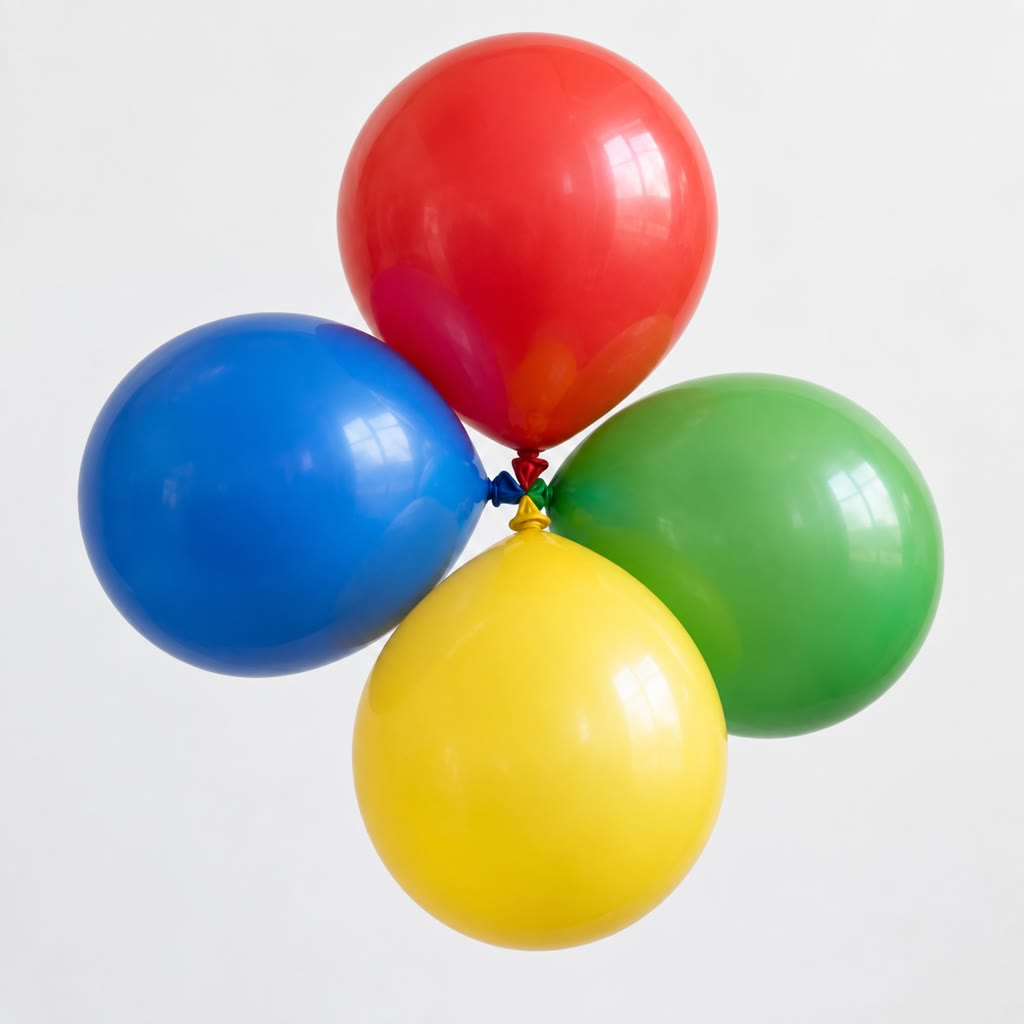
\includegraphics[width=0.38\linewidth]{images/book1/ai/g10-balloons-tetrahedron.jpg}

{\small Quatro balões amarrados juntos se empurram o mais longe possível
uns dos outros; no espaço, eles apontam para os vértices de um
tetraedro, como os quatro pares de \omterm{def:g9:inside-the-atom:nucleus}{elétrons} em volta de um \omterm{def:g7:atoms-and-molecules:atom}{átomo} de
carbono.}
\end{omfigure}

\section{Desenhar as moléculas no espaço}

\begin{notation}[Cunhas cheias e tracejadas]\label{not:g10:lewis-and-shape:wedge}
Para desenhar uma \omterm{def:g7:atoms-and-molecules:molecule}{molécula} no espaço num papel plano, uma ligação no
plano do papel é um traço simples, uma ligação que aponta para o leitor
é uma cunha cheia, e uma ligação que se afasta dele é uma cunha
tracejada. O metano é então desenhado como abaixo: duas ligações no
plano, uma voltada para o leitor e uma voltada para trás.
\begin{center}
\chemfig{C(-[2]H)(-[4]H)(<[7]H)(<:[5]H)}
\end{center}
\end{notation}

\section{Exercícios}

\begin{exercise}[$\star$]\label{exo:g10:lewis-and-shape:1}
O que é uma \omterm{def:g10:lewis-and-shape:covalent-bond}{ligação covalente}? O que é um \omterm{def:g10:lewis-and-shape:lone-pair}{par não ligante}?
\end{exercise}

\begin{exercise}[$\star$]\label{exo:g10:lewis-and-shape:2}
Quantas \omterm{def:g10:lewis-and-shape:covalent-bond}{ligações covalentes} o hidrogênio, o carbono, o nitrogênio e o
oxigênio costumam formar? Explique com as \omterm{def:g10:electron-shells:octet}{regras do octeto} e do dueto.
\end{exercise}

\begin{exercise}[$\star$]\label{exo:g10:lewis-and-shape:3}
Desenhe a \omterm{def:g10:lewis-and-shape:lewis-structure}{estrutura de Lewis} do cloreto de hidrogênio, \ce{HCl}, e conte
os \omterm{def:g9:inside-the-atom:nucleus}{elétrons} em volta do cloro.
\end{exercise}

\begin{exercise}[$\star$]\label{exo:g10:lewis-and-shape:4}
Quantos \omterm{def:g10:electron-shells:valence}{elétrons de valência}, ao todo, tem a \omterm{def:g7:atoms-and-molecules:molecule}{molécula} \ce{NH3}? Quantos
pares?
\end{exercise}

\begin{exercise}[$\star$]\label{exo:g10:lewis-and-shape:5}
Dê a geometria de \ce{CH4}, \ce{NH3}, \ce{H2O} e \ce{CO2}.
\end{exercise}

\begin{exercise}[$\star\star$]\label{exo:g10:lewis-and-shape:6}
Desenhe a \omterm{def:g10:lewis-and-shape:lewis-structure}{estrutura de Lewis} do sulfeto de hidrogênio, \ce{H2S} (o
enxofre está no grupo do oxigênio), e preveja a sua geometria.
\end{exercise}

\begin{exercise}[$\star\star$]\label{exo:g10:lewis-and-shape:7}
Desenhe a \omterm{def:g10:lewis-and-shape:lewis-structure}{estrutura de Lewis} do nitrogênio, \ce{N2}, seguindo o método
passo a passo.
\end{exercise}

\begin{exercise}[$\star\star$]\label{exo:g10:lewis-and-shape:8}
Desenhe a \omterm{def:g10:lewis-and-shape:lewis-structure}{estrutura de Lewis} do metanol, \ce{CH3OH}, e dê a geometria
em volta do carbono e em volta do oxigênio.
\end{exercise}

\begin{exercise}[$\star\star$]\label{exo:g10:lewis-and-shape:9}
Por que o \ce{CO2} é linear e o \ce{H2O} é angular, se os dois têm um
\omterm{def:g7:atoms-and-molecules:atom}{átomo} central ligado a dois outros?
\end{exercise}

\begin{exercise}[$\star\star$]\label{exo:g10:lewis-and-shape:10}
Desenhe a \omterm{def:g10:lewis-and-shape:lewis-structure}{estrutura de Lewis} do eteno, \ce{C2H4}, e dê a geometria em
volta de cada \omterm{def:g7:atoms-and-molecules:atom}{átomo} de carbono.
\end{exercise}

\begin{exercise}[$\star\star$]\label{exo:g10:lewis-and-shape:11}
Desenhe a \omterm{def:g10:lewis-and-shape:lewis-structure}{estrutura de Lewis} do tetraclorometano, \ce{CCl4}, e preveja a
sua geometria.
\end{exercise}

\begin{exercise}[$\star\star\star$]\label{exo:g10:lewis-and-shape:12}
Duas \omterm{def:g7:atoms-and-molecules:molecule}{moléculas} têm a fórmula \ce{C2H6O}. Desenhe uma \omterm{def:g10:lewis-and-shape:lewis-structure}{estrutura de Lewis}
para cada uma (uma tem uma ligação O--H, a outra uma cadeia C--O--C).
\end{exercise}

\begin{exercise}[$\star\star\star$]\label{exo:g10:lewis-and-shape:13}
Explique, usando os \omterm{def:g10:lewis-and-shape:lone-pair}{pares não ligantes}, por que o ângulo da amônia
(\ang{106.7}) é menor que o do metano (\ang{109.5}), e o da água
(\ang{104.5}) menor ainda.
\end{exercise}

\begin{exercise}[$\star\star\star$]\label{exo:g10:lewis-and-shape:14}
Desenhe a \omterm{def:g10:lewis-and-shape:lewis-structure}{estrutura de Lewis} do cianeto de hidrogênio, \ce{HCN}, e a do
metanal, \ce{CH2O}, e dê as suas geometrias.
\end{exercise}

\begin{exercise}[$\star\star\star$]\label{exo:g10:lewis-and-shape:15}
O ozônio, \ce{O3}, é uma cadeia de três \omterm{def:g7:atoms-and-molecules:atom}{átomos} de oxigênio. Conte os
seus pares de valência e desenhe uma \omterm{def:g10:lewis-and-shape:lewis-structure}{estrutura de Lewis} em que cada
oxigênio tenha um octeto (uma \omterm{def:g10:lewis-and-shape:multiple-bond}{ligação dupla}, uma ligação simples).
Preveja se a \omterm{def:g7:atoms-and-molecules:molecule}{molécula} é linear ou angular.
\end{exercise}

\section{Problema: uma molécula num cubo}

\begin{problem}[{Problema de fim de semana --- projetar as bolas de
carbono de um kit de modelos moleculares: em que ângulo os furos devem
ser feitos?}]
\label{pb:g10:lewis-and-shape:1}
% ledger: ang:H2O, ang:NH3
Uma empresa fabrica kits de modelos moleculares. As bolas pretas de
carbono têm de ter quatro furos, para que o metano, o etano e as outras
\omterm{def:g7:atoms-and-molecules:molecule}{moléculas} do carbono saiam com a forma certa. O engenheiro usa um
truque: um tetraedro regular cabe dentro de um cubo, com os seus quatro
vértices em quatro vértices do cubo, sem que dois deles fiquem na mesma
aresta.

\medskip
\noindent\textbf{Parte I --- \omterm{def:g10:lewis-and-shape:lewis-structure}{Estruturas de Lewis}.}
\begin{enumerate}
  \item Desenhe as \omterm{def:g10:lewis-and-shape:lewis-structure}{estruturas de Lewis} do metano \ce{CH4}, da amônia
        \ce{NH3} e da água \ce{H2O}.
  \item Quantos grupos de \omterm{def:g9:inside-the-atom:nucleus}{elétrons} cercam o \omterm{def:g7:atoms-and-molecules:atom}{átomo} central em cada uma?
  \item Quantos deles são \omterm{def:g10:lewis-and-shape:lone-pair}{pares não ligantes}?
  \item Por que uma bola de carbono precisa de quatro furos, e uma bola
        de oxigênio (para a água) só de dois?
  \item Um modelo do etano, \ce{C2H6}, usa duas bolas de carbono.
        Desenhe a sua \omterm{def:g10:lewis-and-shape:lewis-structure}{estrutura de Lewis}. Quantas varetas ligam as duas
        bolas de carbono, e quantas bolas de hidrogênio são necessárias?
\end{enumerate}

\medskip
\noindent\textbf{Parte II --- Geometrias.}
\begin{enumerate}[resume]
  \item Dê a geometria de cada uma das três \omterm{def:g7:atoms-and-molecules:molecule}{moléculas}.
  \item Os ângulos medidos são \ang{106.7} na amônia e \ang{104.5} na
        água. Explique por que eles são menores que o ângulo do metano.
  \item Por que a bola de oxigênio para a água não pode ser simplesmente
        uma bola de carbono com dois furos vazios, se o kit deve mostrar
        o ângulo verdadeiro?
  \item No dióxido de carbono, o \omterm{def:g7:atoms-and-molecules:atom}{átomo} de carbono forma duas \omterm{def:g10:lewis-and-shape:multiple-bond}{ligações
        duplas}. Que ângulo deve separá-las num modelo?
\end{enumerate}

\medskip
\noindent\textbf{Parte III --- O cubo.}
Tome um cubo de aresta $a$. O \omterm{def:g7:atoms-and-molecules:atom}{átomo} de carbono está no centro dele; os
quatro \omterm{def:g7:atoms-and-molecules:atom}{átomos} de hidrogênio ficam em quatro vértices do cubo, sem que
dois deles fiquem na mesma aresta.
\begin{enumerate}[resume]
  \item Mostre que dois quaisquer desses \omterm{def:g7:atoms-and-molecules:atom}{átomos} de hidrogênio estão nas
        duas extremidades de uma diagonal de uma face do cubo. Usando o
        teorema de Pitágoras, calcule a distância entre eles em função
        de $a$.
  \item A diagonal do cubo inteiro (de um vértice ao vértice oposto) tem
        comprimento $a\sqrt{3}$. Deduza a distância do \omterm{def:g7:atoms-and-molecules:atom}{átomo} de carbono a
        um \omterm{def:g7:atoms-and-molecules:atom}{átomo} de hidrogênio.
  \item Tome $a = \qty{1}{cm}$ num modelo: dê as duas distâncias em
        centímetros, com duas casas decimais.
  \item Por que as quatro distâncias C--H são iguais?
\end{enumerate}

\medskip
\noindent\textbf{Parte IV --- O ângulo.}
O \omterm{def:g7:atoms-and-molecules:atom}{átomo} de carbono C e dois \omterm{def:g7:atoms-and-molecules:atom}{átomos} de hidrogênio H$_1$, H$_2$ formam um
triângulo isósceles. Seja M o ponto médio de H$_1$H$_2$.
\begin{enumerate}[resume]
  \item Explique por que o triângulo C\,M\,H$_1$ tem um ângulo reto em M.
  \item Calcule, nesse triângulo retângulo, o seno do ângulo
        $\widehat{\text{M\,C\,H}_1}$, metade do ângulo H--C--H.
  \item Deduza o meio ângulo, e depois o ângulo H--C--H, com uma casa
        decimal.
  \item Compare com o ângulo da tabela deste capítulo.
  \item Dê o ângulo segundo o qual os furos de uma bola de carbono devem
        ser feitos.
\end{enumerate}
\end{problem}
